\newif\ifglobal

%%%%%%%%%%%%%%%%%%%%%%%
%%% Compile to view %%%
%%%%%%%%%%%%%%%%%%%%%%%

%%%%%%%%%%%%%%%%%%%%%%%%%%%%%%%%%%%%%%%%%%%%%%%%%%%
%%% Readme:                                     %%%
%%% https://www.overleaf.com/read/bwdjvfjksvjy/ %%%
%%%%%%%%%%%%%%%%%%%%%%%%%%%%%%%%%%%%%%%%%%%%%%%%%%%

% >>> M?: marks a module setting number or important notice

% >>> M4: Set {./relative-path} to external files for this module <<<
\def \modulefiles {./02-DMA}
% To add an external file, use:
% (Replace '---' with actual filename)
% '\input{\modulefiles/tables/---.tex}' for tables
% '\includegraphics{\modulefiles/figures/---}' for figures
% '\subfile{\modulefiles/---}' for register files


% >>> M1: This module is in global project? <<<
% 'YES' - uncomment; 'NO' - comment out
\globaltrue

\ifglobal
    \documentclass[main\_\_CN.tex]{subfiles}

\else
    % Font "FandolSong-Regular" used by ctex does not have GSUB table.
    % It causes warnings that do not affect compilation and can be ignored.
    \PassOptionsToPackage{quiet}{fontspec}

    \documentclass[openany, 10pt]{book}

    % >>> M2: In ./00-shared/preamble-trm-module, also find
    %         settings for visibility of todo notes, watermark <<<
    \usepackage{preamble-trm-module}


    % Enable Chinese typesetting
    \usepackage{ctex}

    % >>> M3: Temporary labels in Chinese
    %         you can add your own labels there <<<
    \myexternaldocument{./00-shared/temp-labels-cn}

\fi %\ifglobal


\setcounter{secnumdepth}{4}

% Define formatting of chapters in text
\setchineseformatting

% >>> M5: If this module needs any updates in
% './00-shared/preamble-trm-module.sty'
% (include additional package, etc.), contact your module PM
% or create the file './00-shared/changelog.tex' make the
% necessary updates yourself and document them in this file <<<

% Make text left-aligned and allow latex to break pages naturally, comment out for full justification
\raggedright
\raggedbottom


\begin{document}

\hypertarget{dma}{}
\chapter{DMA 控制器 (DMA)}\label{mod:dma}

\section{概述}

直接存储访问 (Direct Memory Access, DMA) 用于在外设与存储器之间以及存储器与存储器之间提供高速数据传输。可以在无需任何 CPU 操作的情况下通过 DMA 快速移动数据，从而提高了 CPU 的效率。

ESP32 中有以下外设具有 DMA 功能：
\begin{itemize}
    \item 三个 UART 接口，即 UART0、UART1 和 UART2，使用 \nameref{sec:UDMA}。
    \item 三个 SPI 接口，即 SPI1、SPI2 和 SPI3，使用 \nameref{sec:dma-spi-dma}。
    \item 两个 I2S 接口，即 I2S0 和 I2S1，使用 \nameref{sec:dma-i2s-dma}。
        \begin{tiplisting}
            ADC 控制器可通过 I2S 接口使用 DMA，详见章节 \nameref{sec:i2s-adc-dac}。
        \end{tiplisting}
    \item SDIO 从机接口，使用章节 \nameref{mod:sdioslave} 中描述的专用 DMA。
    \item SD/MMC 主机接口，使用章节 \nameref{mod:sdhost} 中描述的专用 DMA。
    \item 以太网 MAC (EMAC) 接口，使用章节 \nameref{mod:ethernetmac} 中描述的专用 DMA。
    \item 蓝牙 (BT)。
    \item Wi-Fi。
\end{itemize}


\section{特性}

DMA 控制器具有以下几个特点：

\begin{itemize}
    \item AHB 总线架构
    \item 支持半双工和全双工收发数据
    \item 数据传输以字节为单位，传输数据量可软件编程
    \item 支持 4-beat burst 传输
    \item 328 KB DMA 地址空间
    \item 通过 DMA 实现高速数据传输
\end{itemize}

\section{功能描述}

ESP32 中所有需要进行高速数据传输的模块都具有 DMA 功能。DMA 控制器与 CPU 的数据总线使用相同的地址空间访问内部 RAM。

根据各自模块的需求，各个模块的 DMA 控制器 功能有所差别，但是 DMA 引擎 (DMA\_ENGINE) 的结构相同。

\subsection{DMA 引擎 的架构}

\begin{figure}[H]
\fbox{
\includegraphics[width=0.5\textwidth]{./02-DMA/figures/DMA_ENGINE}}
\centering
\caption{DMA 引擎 的架构}
\label{Figure:DMA_ENGINE}
\end{figure}

DMA 引擎 通过 AHB\_BUS 将数据存入内部 RAM 或者将数据从 RAM 取出。图 \ref{Figure:DMA_ENGINE} 为 DMA 引擎 基本架构图。其中 RAM 为 ESP32 的内部 SRAM，SRAM 的具体使用范围详见章节 \ref{mod:sysmem} \textit{\nameref{mod:sysmem}}。软件可以通过挂载链表的方式来使用 DMA 引擎。DMA\_ENGING 根据 out\_link 中的内容将相应 RAM 中的数据发送出去，也可根据 in\_link 中的内容将接收的数据存入指定 RAM 地址空间。

\subsection{链表}

\begin{figure}[H]

\includegraphics[width=0.5\textwidth]{./02-DMA/figures/link_descriptor}
\centering
\caption{链表结构图}
\label{Figure:link_descriptor}
\end{figure}

out\_link 与 in\_link 结构相同，图 \ref{Figure:link_descriptor} 所示为链表的结构图，一个链表由 3 个字组成。每一字段的意义如下：

\begin{itemize}
    \item owner (DW0) [31]：表示当前链表对应的 buffer 允许的操作者。\\
    1'b0：允许的操作者为 CPU；\\
    1'b1：允许的操作者为 DMA 控制器。
    \item eof (DW0) [30]：表示结束标志。\\
    1'b0：当前链表不是最后一个链表；\\
    1'b1：当前链表为数据包的最后一个链表。
    \item reserved (DW0) [29:24]：reserved。\\
    软件不能写 1。
    \item length (DW0) [23:12]：表示当前链表对应的 buffer 中的有效字节数。从 buffer 中读取数据时表示能够读取的字节数；向 buffer 中存储数据时表示已存数据的字节数。
    \item size (DW0) [11:0]：表示当前链表对应的 buffer 的大小。\\
       {\bfseries 注意}：大小必须字对齐。
    \item buffer address pointer (DW1)：buffer 地址指针。\\
    {\bfseries 注意}：地址必须字对齐。
    \item next descriptor address (DW2)：下一个链表的地址指针。当前链表为最后一个链表时 (eof=1)，该值为 0。
\end{itemize}

用 DMA 接收数据时，如果一帧数据长度小于给定的 buffer 长度，那么 DMA 不会接着使用这个 buffer 剩余空间。这使得 DMA\_ENGING 可以用于传输任意字节数的数据。

\section{UART DMA (UDMA) 控制器}\label{sec:UDMA}

ESP32 中有 3 个 UART 接口，它们共用 2 个 UDMA 控制器。UHCI\_UART\textcolor{red}{\it{x}}\_CE（\textcolor{red}{\it{x}} 为 0、 1、2）寄存器用于选择哪一个 UART 使用当前的 UDMA。

\begin{figure}[H]

\includegraphics[width=0.5\textwidth]{./02-DMA/figures/UDMA}
\centering
\caption{UDMA 模式数据传输}
\label{Figure:UDMA}
\end{figure}

图 \ref{Figure:UDMA} 为 UDMA 方式数据传输图。在接收数据前，软件将接收链表准备好。UHCI\_INLINK\_ADDR 用于指向第一个 in\_link 链表。寄存器必须配置接收链表的低 20 位地址。 置位 UHCI\_INLINK\_START 之后，通用主机控制器接口 (UHCI) 会将 UART 接收到的数据传送给 Decoder。经过 Decoder 解析之后的数据在 DMA 引擎 的控制下存入接收链表指定的 RAM 空间。

在发送数据前，软件需要将发送链表和发送数据准备好，UHCI\_OUTLINK\_ADDR 用于指向第一个 out\_link 链表。 寄存器必须配置发送链表的低 20 位地址。置位 UHCI\_OUTLINK\_START 之后，DMA 引擎 即从链表中指定的 RAM 地址读取数据，并通过 Encoder 进行数据包封装，然后经 UART 的发送模块串行发送出去。

UART DMA 的数据包格式为（分隔符+数据+分隔符）。Encoder 用于在数据前后加上分隔符，并将数据中和分隔符一样的数据用特殊字符替换。Decoder 用于去除数据包前后分隔符，并将数据中的特殊字符进行替换为分隔符。数据前后的分隔符可以有连续多个。分隔符可由 UHCI\_SEPER\_CHAR 进行配置，默认值为 0xC0。数据中与分隔符一样的数据可以用 UHCI\_ESC\_SEQ0\_CHAR0（默认为 0xDB）和 UHCI\_ESC\_SEQ0\_CHAR1（默认为0xDD）进行替换。当数据全部发送完成后，会产生 UHCI\_OUT\_TOTAL\_EOF\_INT 中断。当数据接收完成后，会产生 UHCI\_IN\_SUC\_EOF\_INT 中断。

\begin{tiplisting}
需要注意的是，接收链表描述符的参数 buffer address pointer 需要按字对齐，并且最后一个描述符的参数 size 需要至少比接收的数据长度大 4 字节。
\end{tiplisting}

\section{SPI DMA 控制器}\label{sec:dma-spi-dma}

\begin{figure}[H]
\fbox{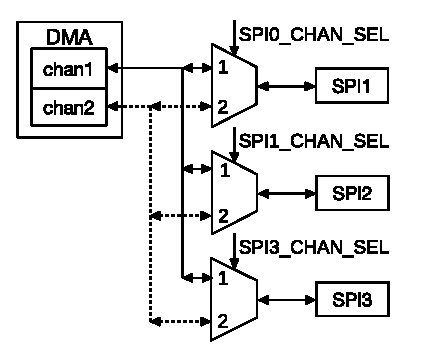
\includegraphics[width=0.45\textwidth]{./02-DMA/figures/SPI_DMA}}
\centering
\caption{SPI DMA}
\label{Figure:SPI_DMA}
\end{figure}

ESP32 SPI 除了使用 CPU 实现与外设的数据交换外，还可以使用 DMA 。如图 \ref{Figure:SPI_DMA} 所示，共有两个 DMA 通道可供 SPI1、SPI2 和 SPI3 控制器选择，每个 DMA 通道可供一个 SPI 控制器使用，即每次可以有两个 SPI 控制器同时使用 DMA。

ESP32 SPI DMA 使用链表接收/发送数据，发送数据支持 burst 操作，一次接收/发送的数据长度应当与 4 字节对齐， 以确保正确收发数据。SPI DMA 支持连续收发数据。

配置 DPORT\_SPI\_DMA\_CHAN\_SEL\_REG 寄存器的 SPI1\_DMA\_CHAN\_SEL[1:0]、 SPI2\_DMA\_CHAN\_SEL[1:0] 和 SPI3\_DMA\_CHAN\_SEL[1:0] 三个域以使能 SPI DMA 接口。每个 SPI 控制器对应一个域，每个域有 2 比特，对应取值为 0、1 和 2， 而不可以取 3 。

以 SPI1 为例，\\
若 SPI1\_DMA\_CHAN\_SEL[1:0] = 0，那么 SPI1 不使用 DMA 通道；\\
若 SPI1\_DMA\_CHAN\_SEL[1:0] = 1，那么 SPI1 使能 DMA 通道 1； \\
若 SPI1\_DMA\_CHAN\_SEL[1:0] = 2，那么 SPI1 使能 DMA 通道 2。

寄存器 SPI\_DMA\_OUT\_LINK\_REG 的 SPI\_OUTLINK\_START 比特和寄存器 SPI\_DMA\_IN\_LINK\_REG 的 SPI\_INLINK\_START 比特用于使能 DMA 引擎，这两个比特由硬件清零。当 SPI\_OUTLINK\_START 比特被置为 1 时，DMA 引擎 开始处理发送链表，并准备发送数据；当 SPI\_INLINK\_START 比特被置为 1 时， DMA 引擎 开始处理接收链表，并准备接收数据。

SPI\_DMA 接口的软件配置流程如下：
\begin{enumerate}
    \item 首先复位 DMA 状态机和 FIFO 指针；
\item 配置 DMA 相关寄存器；
\item 配置 SPI 接口相关寄存器；
\item 使能一次 DMA 操作。
\end{enumerate}

\section{I2S DMA 控制器}\label{sec:dma-i2s-dma}

ESP32 有两个 I2S 接口，即 I2S0 和 I2S1。 I2S0 和 I2S1 各有一个 DMA 通道。寄存器 I2S\_FIFO\_CONF\_REG 的 REG\_I2S\_DSCR\_EN 比特用于使能 I2S 的 DMA 操作。ESP32 I2S DMA 使用链表接收/发送数据，发送数据支持 burst 操作，一次接收/发送的数据长度为 1 个字（4 个字节）。 寄存器 I2S\_RXEOF\_NUM\_REG 的 REG\_I2S\_RX\_EOF\_NUM[31:0] 比特用于配置 DMA 一次接收数据长度，单位为字。

寄存器 I2S\_OUT\_LINK\_REG 的 I2S\_OUTLINK\_START 比特和寄存器 I2S\_IN\_LINK\_REG 的 I2S\_INLINK\_START 比特用于使能 DMA 引擎，这两个比特由硬件清零。 当 I2S\_OUTLINK\_START 比特被置为 1 时， DMA 引擎 开始处理发送链表，并准备发送数据，当 I2S\_INLINK\_START 比特被置为 1 时， DMA 引擎 开始处理接收链表，并准备接收数据。

I2S DMA 接口的软件配置流程如下：
\begin{enumerate}
    \item 首先配置 I2S 接口相关寄存器；
   \item  复位 DMA 状态机和 FIFO 指针；
   \item 配置 DMA 相关寄存器；
   \item 在 I2S 主机模式下，设置 I2S\_TX\_START 比特或者 I2S\_RX\_START 比特，发起一次 I2S 操作；\\
   在 I2S 从机模式下，设置 I2S\_TX\_START 比特或者 I2S\_RX\_START 比特后等待主机发起数据传输的请求。
\end{enumerate}
I2S DMA 中断说明详见章节 \ref{mod:i2s} \textit{\nameref{mod:i2s}}，\hyperref[DMA Interrupts]{DMA 中断}。
\end{document}
